\begin{comment}
\begin{figure}
   \begin{subfigure}[b]{0.45\textwidth}
    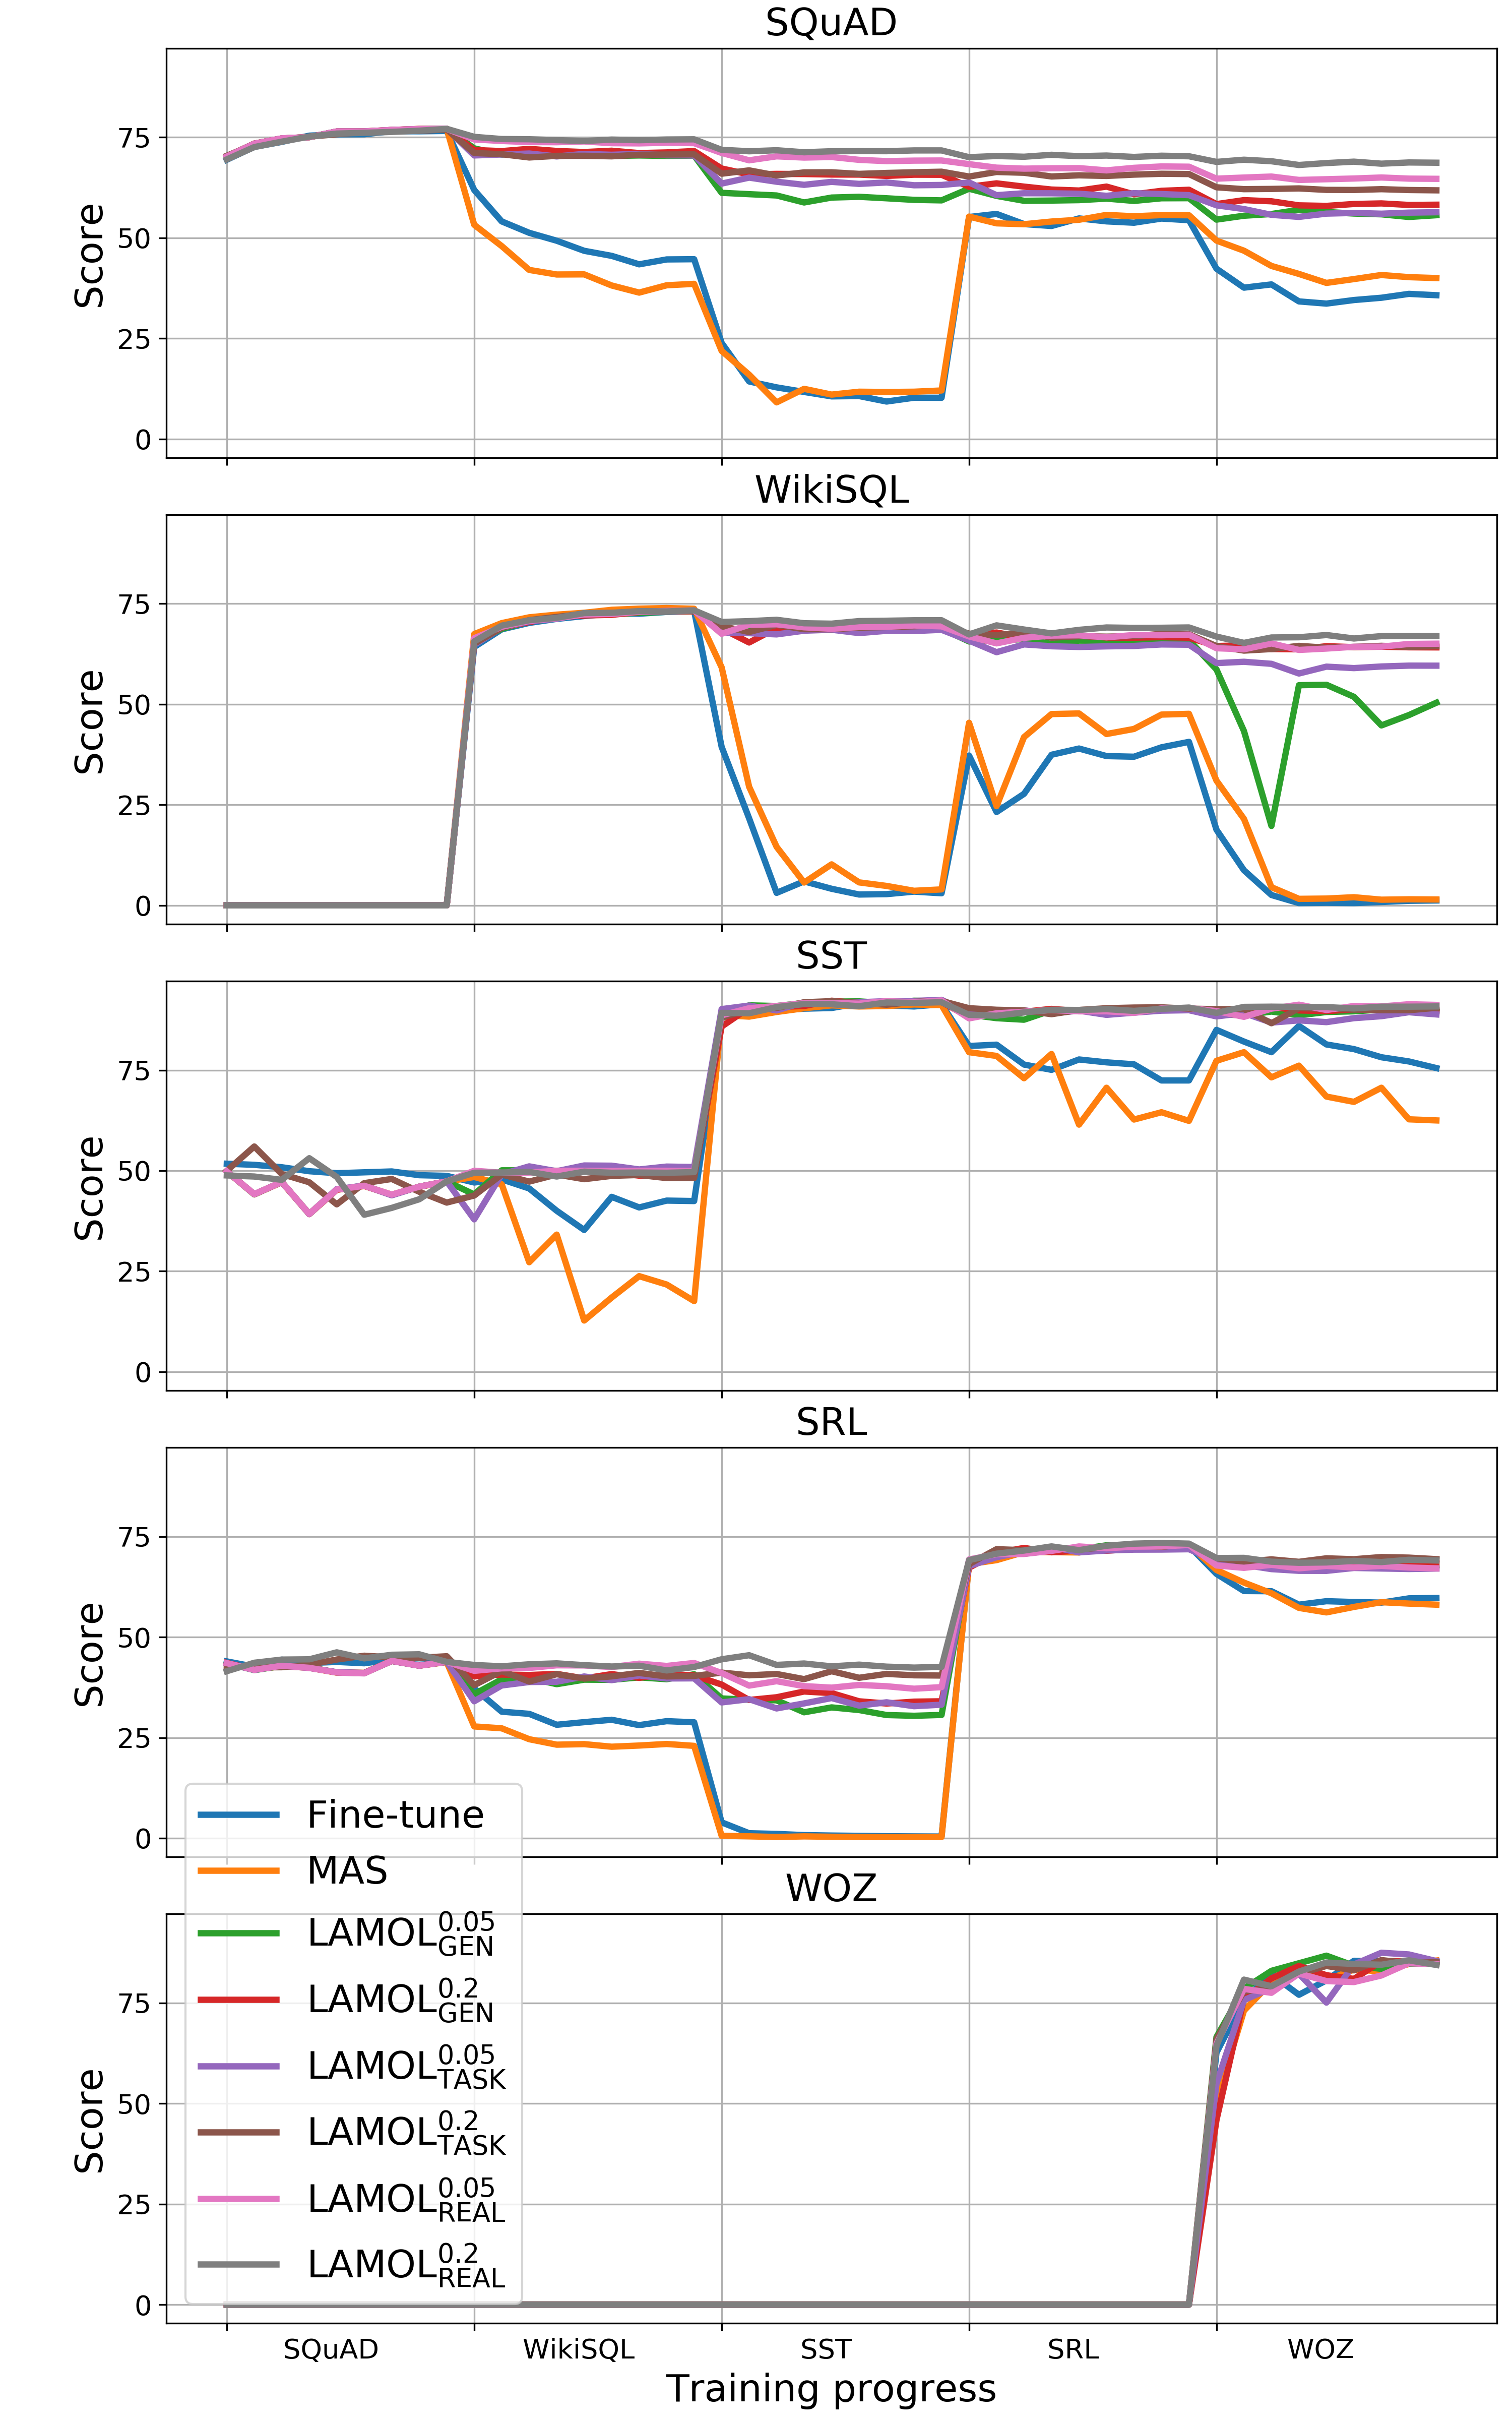
\includegraphics[width=\linewidth,height=1.4\linewidth]{imgs/five_tasks.png}
    \caption{Training progress of five tasks. The graph records the performance of the model at each epoch of each task.
%   The order of task orders in the progress follows: 
    The task order is    % AMH: check
    SQuAD, WikiSQL, SST, QA-SRL and then WOZ.}
    \label{fig:five_tasks}
   \end{subfigure}
   \hfill
   \begin{subfigure}[b]{0.45\textwidth}
    
\includegraphics[width=\linewidth,height=1.4\linewidth]{imgs/cmp_gen_size.png}
    \caption{Performance after each epoch under five different sampling ratios, with or without task specific-specific tokens. In total, ten combinations are tested on WikiSQL, SST, QA-SRL, and WOZ.}
    \label{fig:cmp_gen_size}
   \end{subfigure}
\end{figure}
\end{comment}

\begin{figure}[!t]
    \begin{minipage}{.45\textwidth}
        \centering
        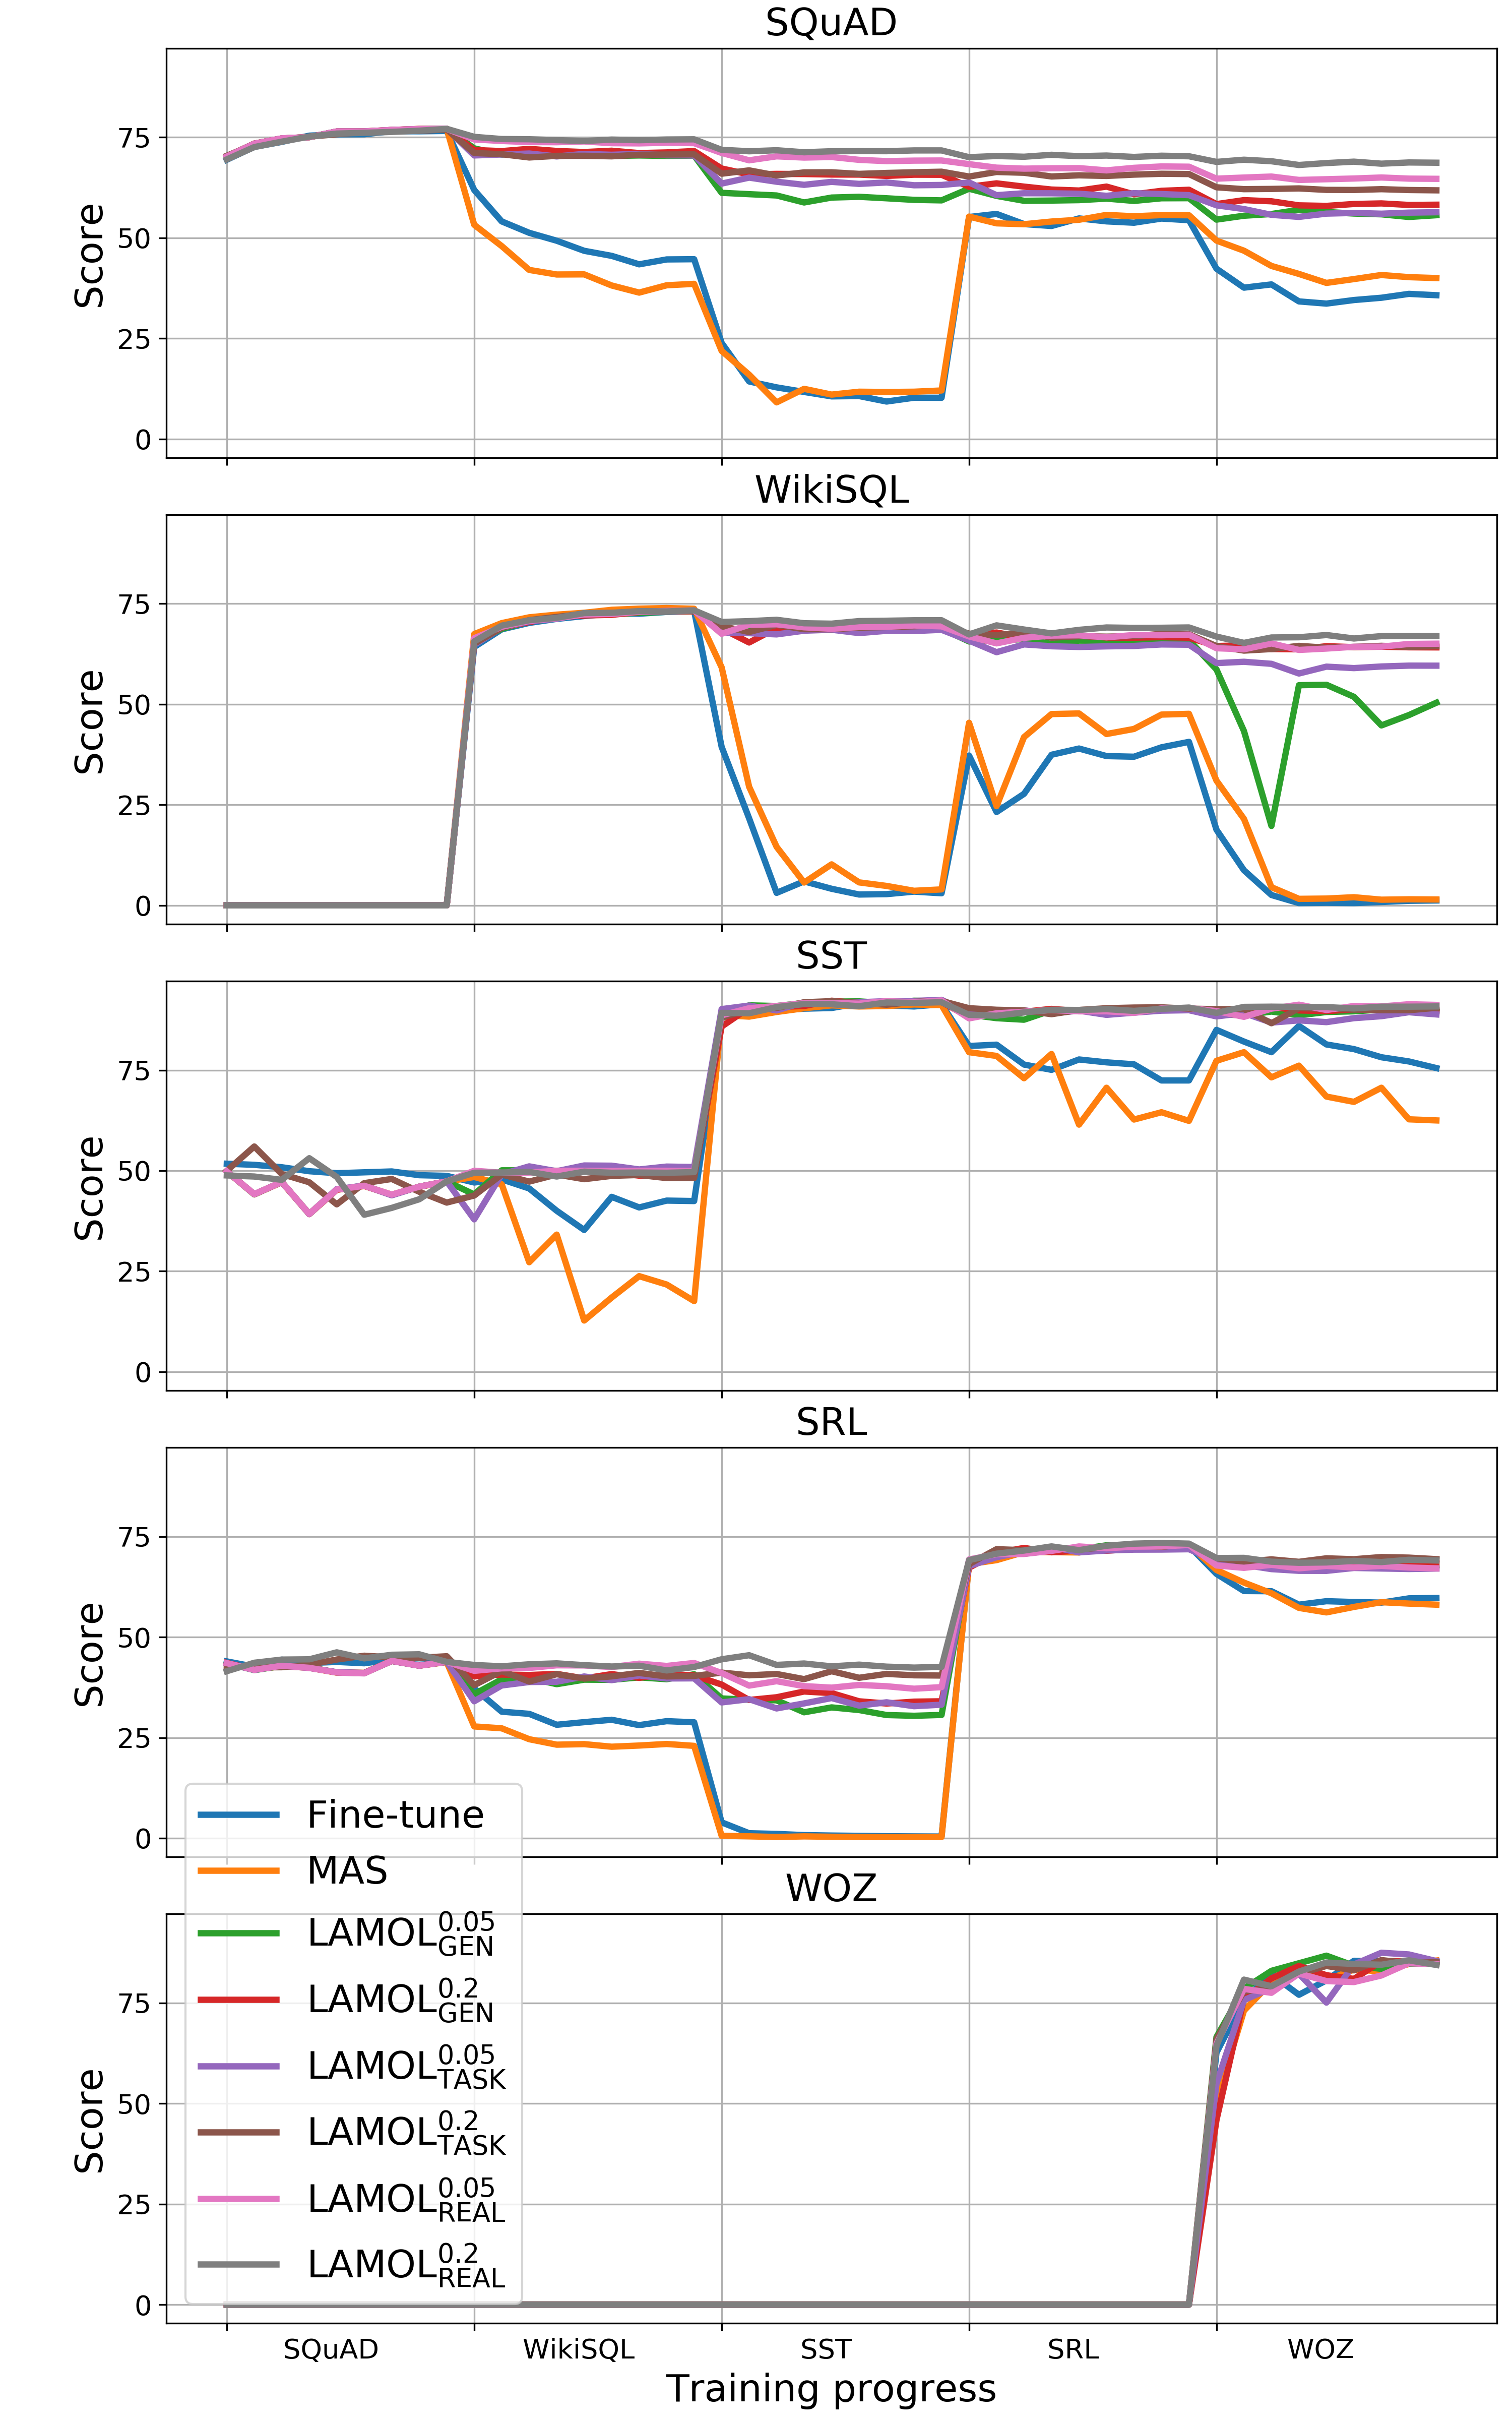
\includegraphics[width=\linewidth]{imgs/five_tasks.png}
        \caption{Training progress of five tasks. The graph records the performance of the model at each epoch of each task.}
        \label{fig:five_tasks}
    \end{minipage}\hfill
    \begin{minipage}{.52\textwidth}
        \centering
        
\includegraphics[width=\linewidth]{imgs/cmp_gen_size.png}
        \caption{Performance after each epoch under five different sampling ratios, with or without task specific-specific tokens.}
        \label{fig:cmp_gen_size}
    \end{minipage}
\end{figure}